% Submit to Electronic Journal of eGovernment http://www.ejeg.com/index.htm %
% Chapter 2 of my dissertation

\documentclass{article}
\usepackage{times}
\usepackage[margin=1in]{geometry}
\usepackage{ifpdf}

\ifpdf
 \usepackage[pdftex]{graphicx}
\else
 \usepackage{graphicx}
\fi

\usepackage{xspace}
\usepackage{tabularx}
\usepackage{epsfig}
\usepackage{amsmath}
\usepackage{amsfonts}
\usepackage{amssymb}
\usepackage{eucal}
\usepackage{float}
\usepackage{times}

\ifpdf
 \usepackage[pdftex,bookmarks=false,a4paper=false,
            plainpages=false,naturalnames=true,
            colorlinks=true,pdfstartview=FitV,
            linkcolor=blue,citecolor=blue,urlcolor=blue, pdfauthor="Dermot
            Cochran and Joseph R. Kiniry"]{hyperref}
\else
 \usepackage[dvips,linkcolor=blue,citecolor=blue,urlcolor=blue]{hyperref}
\fi

\usepackage{listings}

% Consistent use of e.g., i.e., etc.
\newcommand{\eg}{e.g.,\xspace}
\newcommand{\ie}{i.e.,\xspace}
\newcommand{\etc}{etc.\xspace}
\def\votail{V\'{o}t\'{a}il\xspace} 
\def\eireann{\'{E}ireann\xspace}
\def\dail{D\'{a}il\xspace}

\newcommand{\myhref}[2]{\href{#1}{#2}} % \myhref as href
\newcommand{\hreffootnote}[3]{\href{#1}{#2}\footnote{#3 \href{#1}{#1}}}

\newcommand{\notej}[1]{\xspace$\frac{\varocircle}{\textsf{jk}}$\marginpar{\scriptsize\textsf{Joe:} #1}}

\begin{document}

\date{}
\title{\votail PRSTV: Ballot Counting Software for Irish Elections} 
\author{
Dermot Cochran\\
IT University of Copenhagen, Denmark\\
dero@itu.dk\\
\and
Joseph R. Kiniry\\
IT University of Copenhagen, Denmark\\
kiniry@acm.org}

\maketitle

% ===========
\begin{abstract}

\votail PRSTV, is an open source Java implementation of 
Ireland's Proportional Representation by Single Transferable Vote (PRSTV)
method of voting, which meets the requirements laid down by Ireland's former
Commission on Electronic Voting. \votail has developed by making a formal
analysis of the ballot counting requirements, expressed in the Java Modeling
Language (JML).

\end{abstract}

%===============
\section{Introduction}

\subsection{Electronic Voting in Ireland}

\subsubsection{Recent History}
The Irish government recently
decided to save costs by disposing of its current generation of direct recording electronic (DRE) voting machines.  The decision to stop using electronic voting was due to mixture of technical issues with regard to the actual voting machines in addition to more general concerns about the security of electronic voting.  The current political consensus is that electronic voting (in its 
current form e.g. DRE machines) will not be used in the Republic of Ireland. 

\paragraph{The IES Software}

An independant test of the IES count software \cite{CEVApp2Ept1} found that

\begin{itemize}

\item Divergences in the number of votes allocated to candidates during surplus
distributions were observed in a number of elections.
\item Errors occur as a result of the representation of the transfer factor
\ldots due to the fact that the transfer factor was represented as a floating
point number


\end{itemize}



\subsubsection{What went wrong?}

Electronic Voting has been used in Brazil for over ten years
\cite{rezende2004electronic} \cite{costa2003brazilian}
\cite{michel2005electronic}, so why not in Ireland?

\subsubsection{Possible solutions}

Electronic counting has the potential to eliminate the randomness within the
existing paper-based count process.

Abandon paper-based mixing and numbering of ballots. This has the potential to
bias the vote by putting ones preferred candidate higher in the pile of ballots.

Use fractional transfers. Use the exact fractional quota without rounding up.

Record and reuse the random selection used in any tie breakers, in the event of
multipe ties.

\subsection{Proportional Representation with Single Transferable Vote}

\subsubsection{PRSTV in Ireland}


 
Note that Irish legislation uses the term 'vote' as a noun to mean the contents
of a ballot paper rather than as a verb for the action of casting
a ballot.~\cite{CEV00-16}.

\begin{quote}
For the purpose of clarity, �vote� means the full set of candidate preferences recorded by a voter at an election.
\end{quote}

Oireachtas \eireann (the National Parliament of the Republic of Ireland) has two
chambers of which the dominant \dail \eireann (Irish house of representatives or lower house) is directly elected by the people for a term of up to five years by a quota-based single transferable vote system in multi-seat constituencies.  

The Republic of Ireland uses Proportional Representation by Single Transferable Vote (PR-STV) for its national, local and european elections.  

The political significance of lost, corrupted or altered votes depends on the type of voting system (\eg STV) and the closeness of the election race. In PR-STV, 
it is not unusual to see the final seat in a multi-winner constituency
determined in the last round of counting by a small number of votes.

Manual recounts are often called for closely contested seats, as the results
often vary slightly, indicating small errors in the manual process of counting
votes. Paper based voting with counting by hand is popular in Ireland, and recent
attempts at automation were frustrated by subtle logic errors in the ballot
counting software \cite{Coyle2004}.  The logic errors exist, in part, due to the
complexities and idiosyncrasies with regard to tie breaking and especially the rounding
of vote transfers. Soem of these relate to the rounding up or down of ballot
transfers and to the randomisation effect of ballot shuffling. Ballot shuffling
does not have have a precise mathemtical definition. Every ballot and every
preference on a ballot can make a difference when the last seat of a multi-seat
constituency is being decided.

Referenda to introduce plurality voting were rejected twice by the Irish
electorate, in 1959 and again in 1968 \cite{sinnott1995irish}.  Since then there
have been no further legislative proposals to change the voting scheme used in Ireland.

The following are selected quotes from the CEV report on the previous electronic voting system used in Ireland ~\cite{CEV2ndReport}:

\begin{itemize}
\item Design weaknesses,
including an error in the implementation of the count rules that could compromise the accuracy of
an election, have been identified and these have reduced the Commission's confidence in this
software.

\item The achievement of the full potential of the chosen system in terms of secrecy and accuracy
depends upon a number of software and hardware modifications, both major and minor, and
more significantly, is dependent on the reliability of its software being adequately proven.

\item Taking account of the ease and relative cost of making some of these modifications, the potential
advantages of the chosen system, once modified in accordance with the Commission's
recommendations, can make it a viable alternative to the existing paper system in terms of secrecy
and accuracy.
\end{itemize}

Cryptographers and security experts naturally tend to focus on the risks of
electronic ballot casting, but accuracy in ballot counting is just as
fundamental, if not even more important, espcecially for advanced vote counting
schemes such as PR-STV.. Manual paper-based counting is perceived as being more
secure, but is potentially more error prone than electronic counting.  This
paper addresses the software engineering challenges of electronic ballot
counting, using Irish PR-STV as the main example.  Note that the proposal to
place anonymous ballots on a public bulletin board, for public counting, cannot
be achieved with PR-STV without a risk of vote signing~\cite{TeagueEtAl08}.

\section{Votail PRSTV Software}

{V}{\'{o}t\'{a}il} is the Irish word for Vote.

\subsection{History}

\subsubsection{Related Work}

\paragraph{KOA}

It was originally intended that Votail be a plugin for the KOA
\cite{KiniryEtAl06} remote voting system.  The last KOA release was in August
2007 and no further releases are planned.

\paragraph{Cian Votail}

Cian Votail is a formaally specified remote voting web interface written by
Jordan Neill based on KOA but rewritten in Java 1.5. It is not the same as the Votail PRSTV system
described in this paper and has not yet been integated with Votail PRSTV.

\cite{neill-formal}

\paragraph{Civitas}

\cite{clarkson2007civitas}

\paragraph{Helios}

\cite{adida2008helios}

\paragraph{Secure Election Transaction}

The Secure Electronic Transaction proctocol developed by Visa and MasterCard
for credit card security never achieved widespread adoption due to its
complexity. Nevertheless it has similar security properties to those used for
electronic voting crytography and might be suitable for use in remote voting
systems \cite{giorgini2003requirement}.

\paragraph{Mobile voting}

Remote voting on a mobile communications device or via mobile broadband, has
additional problems with regard to the handling of signal fading e.g.
robustness and resiliency.

\subsection{Formal Specification of Proportional Respresentation by Single
Transferable Vote}

Ireland's Commission on Electronic Voting laid down several recommendations for future use of electronic voting, including the following:
\begin{itemize}
\item clear definition of requirements and specifications,
\item robust and formal approach to design and development,
\item separation of critical concerns (election management, count rules, vote file, \etc),
\item the appropriate use of open source methods,
\item publication or public inspection of the source code,
\item open public testing of the vote recording software and the vote counting software via an on-line web interface designed to simulate the hardware interfaces of the 
system, and
\item full and formal process of requirements capture and functional specifications for any proposed new system.
\end{itemize}

This leads us to conclude that the next generation of electronic voting systems in Ireland (if any), will be developed in open source using formal methods, 
and that each functional module (\eg ballot counting) will be developed and tested independently.  
In particular it should be possible to develop two or more different implementations of vote counting, yet to get the same results. 
\votail is intended to be a reference implementation, which will be formally guaranteed to give the correct results for any valid set of ballots.

Also, it will be required that each major subsystem will be implemented separately and that any subsystem could be replaced by an equivalent subsystem.

The use of electronic counting would permit the use of fractional transfers and avoid the need for random sub-selection of ballots when distributing a surplus; 
this would help to ensure that the result is closer to the intent of the electorate and avoid the use of drawing lots to resolve ties -- the likelihood of a tie is greatly reduced when fractional votes are possible. 
The specification will allow for both the traditional method of counting \ie simulation of  the manual counting process and for the use of fractional ballots - 
similar to the Seanad electoral system (Gregory Method) in which there are just a few thousand electors. Note that with manual vote counting it is only possible to support
fractional vote transfers with a small electorate; electronic vote counting could have allowed this to be achieved for the whole electorate, but the previous 
(decommissioned)
evoting system did not allow for this possibility.

The \votail specification describes only the ballot counting process and does not rely on assumptions about how the ballots were cast, transmitted, encrypted or stored.

\subsection{Methodology}

The functional requirements are expressed using Business Object Notation (BON), supplemented with diagrams and tables.
BON can be read as a structured natural language, but can also be type checked.  
 
Note that the specification does not rely on any features of Java 1.5 or Java 1.6, so the implementation to date was made in Java 1.4 source code so as to fully exploit the 
existing mature JML toolset (\eg ESCJava2) rather than the newer JML4 plugin with supports Java 1.5 or OpenJML which supports Java 1.6.

Also we currently have a JML specification for JDK 1.4 but not JDK 1.5 or upwards, so as to allow modular verification with regard to the Java 1.4 API - note that we do
not verify the JDK but treat it as trusted third party - this is dangerous so we will seek to minimize our reliance on the JDK by adding a layer of indirection where required 
and to use primitive data structures e.g. arrays where possible, rather than making use of Java collections, for example.

%---------------------------------------------
\subsection{Requirements Analysis}

\subsubsection{Legal Requirements}

\paragraph{Constitutional Law}

Article 16, section 2, subsection 5 of the Irish Constitution states only that:

\begin{quote}
The members [of parliament] shall be elected on the system of proportional representation by means of the single transferable vote.
\end{quote}

which leaves considerable freedom for the electoral law to define the precise means of vote casting and counting.

\paragraph{Electoral Law}

The functional requirements are read from the electoral legislation and CEV guidelines and listed in a table ~\cite{Cochran06} \eg

\begin{itemize}
\item 1	Counting does not begin until all votes are loaded.
\item 2	The total number of first preference votes must remain the same after each count.
\item 3	The [Droop] quota is equal to ((Number of valid votes cast)/(Number of seats being filled + 1)) + 1, ignoring any remainder.
\item 4	Any candidate with a quota or more than a quota of votes, is deemed to be elected.
\item 5	The surplus of an elected candidate is the difference between the quota and his/her total number of votes.
\item 6	The minimum number of votes required for a candidate to secure the return of his/her deposit is one plus one-quarter of a quota based on the total number of 
seats in the constituency.
\item 7	Any elected candidate automatically saves his/her deposit.
\end{itemize}

The full table of functional requirements have been listed elsewhere ~\cite{Cochran06}.

In addition Sections 32-37 relate to the format of the election report:

\begin{quote}
ELECTRONIC COUNTING
POST-COUNT MENU
SECTION 32 : RESULT SHEET IN WORD FORMAT
When clicked, the �Result sheet in Word format� should convert the Post-Count Result
sheet described in section 32 into a Word document in identical format ready for printing
on A4 and larger page sizes. This document should be stored in the system and via
�Explorer�, be capable of being printed and exported to a floppy disk or CD.
\end{quote}

We have chosen not to implement the above requirement, but instead propose to provide the results in a platform-neutral format e.g. 
XML or via an API which can be processed by a separate document generation system to produce whichever format of document is required. It is important to the note that
the process of translating legal or business requirements (as specified by a business analyst or equivalent) into functional requirements needs to be guided by the
principles of good clean software design and architecture, so to remove unnecessary detail, to resolve ambiguities and to discover hidden assumptions which need
to be made explicit and then clarified.

Each of the functional requirements is cross-referenced to the source document by section number, subsection and page number, so that all requirements are traceable.  
The requirements are listed in order of appearance in each source document so that it can be easily seen if any are missing.  
Not all parts of the legislation translate directly into requirements e.g. the requirement to delete invalid votes from the system:

For example, the Department of the Environment's Commentary on Count Rules ~\cite{CEV00} states that:
\begin{quote}
The system should have a facility to remove from the �Votes as mixed and numbered� table a vote
(notably one cast on a voting machine from a postal or special ballot paper) which the court rules is
invalid and should not be included in the count. To do this, there should be a button in the Petitions
menu entitled �Deletion of invalid vote� which when pressed presents a table with the same column
headings as in the �Votes as mixed and numbered� table and one blank row beneath it. The user enters
in that row the preferences recorded on the vote to be removed from the table (he/she she is not
permitted to enter anything in the Mixed Votes No. column). The user then presses a �Find invalid
vote� button and the system searches the �Votes as mixed and numbered� table, finds the vote in
question and enters its Mixed Vote No. in the Mixed Votes No. column of the table where the user
entered the characteristics of the invalid vote. There should also be a �Remove invalid vote� button
which when pressed by the user would, where there is only one vote in the �Votes as mixed and
numbered� table with the characteristics of the invalid vote, remove that vote from the table and
decrease by one the mixed vote numbers of all votes which succeeded it in the original table.
\end{quote}

This requirement is not listed, but instead is treated as a \emph{precondition} to the ballot counting process; 
it is required that the input to the ballot counting sub-system contains only valid ballots.  
It is assumed that other parts of the system e.g. the vote-casting and election management system have provided us with the valid set of votes, 
and of course, we make no assumptions about how the ballots were cast, whether electronic or paper-based, at the polling place or remotely.  
This is part of the modular design by contract.  The software will fulfill the following contract; 
if the input is a valid set of ballots, we will generate a valid set of results according to the requirements of the 1992 Electoral Act, \etc.  

Also, the requirement for mixing and numbering is a side effect of the paper
counting process resulting in a distrortion of the transfers. Electronic
counting allows for the possibility of exact fractional transfers, rather than
transfers of whole ballots, with rounding of votes.

%---------------------------------------------------------------------
\subsection{Architectural Description and Elaboration}

\subsubsection{Business Object Notation}

These semi-formal statements are then elaborated in a 
software architectural description language.  
This provides a precise formal specification which can be refined into a detailed design and yet is readable by non-programmers.  
We use an ADL called ``BON'' to
describe our system at this early stage.  Business Object Notation (BON) is a method and graphical notation for high-level object-oriented analysis and design.
BON is a system specification language akin to UML that differs in several key
respects.  Contrary to UML, BON has a human-readable textual syntax
\cite{paige1999comparison} \cite{paige2002bon}.

\paragraph{BON Diagrams}

These diagrams were created using a BON stencil for OmniGraffle. This stencil
was created to provide a graphic notation for BON when designing software using
a verification centric process, given the mismatch between UML class diagrams and BON.

\paragraph{Major and Minor classes}

In our graphical notation for BON we distinguish between major and minor
classes. Minor classes are classes introduced during refactoring or as helper
classes to the major classes. Major classes represent a business concept such
as Ballot or a Candidate.

 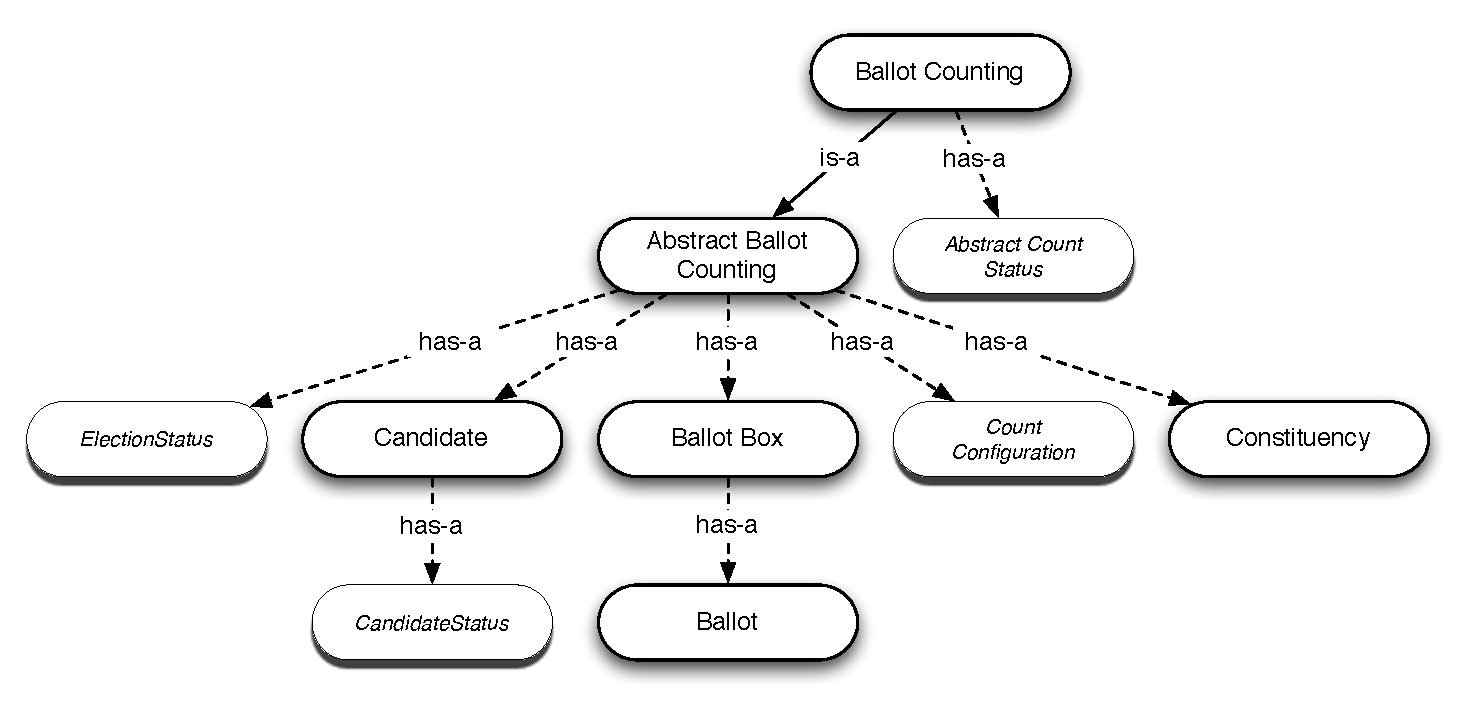
\includegraphics[width=150mm]{Architecture.pdf}

\paragraph{Java Modeling Language}

In the earliest prototype of \votail the JML specifications were taken directly
from the functional requirements. In the current version, the JML
specifications have been refactored and updated to match the BON design.

The Java Modeling Language (JML) is a behavioral interface specification language that can be 
used to specify the behavior of Java modules. It combines the design by contract approach of 
Eiffel and the model-based specification approach of the Larch family of interface specification 
languages, with some elements of the refinement calculus.

\paragraph{BON Description}
\begin{verbatim}
class_chart BALLOT_COUNTING
explanation
  "Count algorithm for tallying of the votes in Dail and Seanad elections"
inherit
  COUNT_PROCESS
query
  "How many continuing candidates?",
  "How many remaining seats?"
command
  "Calculate quota",
  "Find highest continuing candidate with quota",
  "Calculate surplus",
  "Calculate weight factor",
  "Calculate transfer factor",
  "Calculate non-fractional transfers",
  "Calculate fractional differences",
  "Calculate adjustments",
  "Calculate transfers",
  "Move ballots",
  "Weight and transfer ballots",
  "Select lowest continuing candidates for exclusion",
  "Declare remaining candidates elected",
  "Close the count" 
end
\end{verbatim}

\subsection{The Electoral System}

\subsubsection{Examples}

\paragraph{1992 Electoral Act, Section 37}

\begin{itemize}
\item (1) A \dail election shall be conducted in accordance with this Act and,
in case a \dail election is contested, the poll shall be taken according to the
principle of proportional representation, each elector having one transferable
vote.
\item (2) In this section "transferable vote" means a vote which is�
( a ) capable of being given so as to indicate the voter's preference for
the candidates in order, and
( b ) capable of being transferred to the next choice when the vote is
not required to give a prior choice the necessary quota of votes, or
when, owing to the deficiency in the number of the votes given for a
prior choice, that choice is excluded from the list of candidates.
\end{itemize}

\paragraph{Formal Assertions}
Section 37 contains very high level description of the voting system, which is elaborated in more detail by later sections of the act e.g. sections 120-122.  Nevertheless we can immediately derive the following requirements:

\paragraph{The JML Specification}
\begin{verbatim}
{
/**
 * Gets the next preference continuing candidate.
 * 
 * @design This is the nearest next preference i.e.
 * filter the list of preferences to contain continuing candidates and then
 * get the next preference to a continuing candidate, if any.
 * 
 * @param ballot Ballot paper from which to get the next preference
 * 
 * @return Candidate ID of next continuing candidate or NONTRANSFERABLE
 */
/*@ requires state == COUNTING;
  @ ensures (\result == Ballot.NONTRANSFERABLE) <=!=>
  @   (\exists int k; 1 <= k && k <= ballot.remainingPreferences(); 
  @     (\result == ballot.getNextPreference(k)) &&
  @     (\forall int i; 1 <= i && i < k;
  @       isContinuingCandidateID(ballot.getNextPreference(i)) == false)
  @   );
  @*/
}
\end{verbatim}

\subsubsection{The Droop Quota}

\paragraph{1992 Electoral Act, Section 120}

\begin{quote}
(1) The returning officer shall then divide the number of all valid
papers by a number exceeding by one the number of vacancies to be filled; the
result increased by one, any fractional remainder being disregarded, shall be
the number of votes sufficient to secure the election of a candidate and this
number is referred to in this Act as "the quota".
(2) Where at the end of any count the number of votes credited to a
candidate is equal to or greater than the quota, that candidate shall be deemed
to be elected.
\end{quote}

\paragraph{The JML Specification}

\begin{verbatim}
/**
 * Minimum number of votes needed to 
 * guarantee an election.
 */
 //@ public model long quota;
 //@ public invariant 0 <= quota;
 //@ public invariant quota <= totalVotes;
 /**
  * @see requirement 3, section 3, 
  *      item 3, page 13
  */
 /*@ public invariant (PRECOUNT < state) ==> 
   @  quota == 1 + (totalVotes / (seats + 1));
   @*/
\end{verbatim}



%~~~~~~~~~~~~~~~~~~~~~~~~~~~

\section{Conclusion and Future Work}

Existing verification tools are either still under active development or do not yet provide soundness and completeness of verification.  
As yet there is no full functional verification tool which has been fully verified in itself.  Since we can't yet achieve full assurance of verification, 
then we aren't yet ready for electronic voting, except for very low-risk elections for small decentralized organizations in which paper balloting might be 
difficult or uneconomical i.e. in which constituencies cannot be defined by geographic location and postal voting might be unreliable.

Elections are important, counting ballots is only one facet of the entire process, but is a critical component.  Cryptographic verification works with simpler counts such as first-past-the-post.  With PR-STV counting is much more complex and error prone.  In Ireland, it is feasible to count votes by hand due to the smaller population, but the cost of manual counting and of managing paper ballots in a central facility does not scale for larger populations.  Secure storage of ballot boxes in a central facility can become expensive.  STV requires central tallying of ballots.  In Ireland, it is currently less expensive to count votes by hand, than to use commercial proprietary voting machines.  However if Ireland decides to reduce the size of its parliament and therefore increase the size of its constituencies, then manual counting starts to become more expensive.  In practice there is a lot of experience with the manual ballot counting process, but some of the rules for drawing lots, shuffling ballots and rounding of transfers are rendered obsolete by the change of technology, so minor changes in the legislation will be required.  In Ireland the CEV acted as the customer and provided clarifications on request, in line with the standard process for public tenders.  The law was then updated to validate the use of electronic voting and to clarify any such ambiguities.  Similar to banking and tax compliance software, there needs to be provision for updating the software to reflect changes in the law.

Critical systems must be designed and constructed with care and consideration.  Dependable software engineering techniques are appropriate.  If electronic voting is to be used at all, then the software design needs to be flawless.  A typical argument against the use of formal methods is cost and time.  Major elections run every year, at best, so we have the time, and are critical components of our society in which millions are spent on TV advertising alone, so surely we can spend a few tens of thousands of the the critical software component.

Votail was subjected to the same set of independent
tests that were used for the IES system, and it is now publically available at

https://trac.ucd.ie/repos/software/evoting/\votail/releases/beta

%=================
%\bibliographystyle{plain}
%\bibliography{paper}

%=====================================================================
\section{Acknowledgments}

This work is being supported by the IT University of Copenhagen, the European
project Mobius within the IST 6th Framework and national grants from Science
Foundation Ireland including LERO C-SET and LERO Graduate School of Software
Engineering. This paper reflects only the authors' views and the EU is not
liable for any use that may be made of the information contained therein.

%======================================================================
{\footnotesize \bibliographystyle{acm}
  \bibliography{paper}
}

\end{document}


